\documentclass[11pt]{article}
\usepackage[utf8]{inputenc}	% Para caracteres en español
\usepackage{amsmath,amsthm,amsfonts,amssymb,amscd}
\usepackage{multirow,booktabs}
\usepackage[table]{xcolor}
\usepackage{fullpage}
\usepackage{lastpage}
\usepackage{enumitem}
\usepackage{fancyhdr}
\usepackage{mathrsfs}
\usepackage{wrapfig}
\usepackage{setspace}
\usepackage{calc}
\usepackage{multicol}
\usepackage{cancel}
\usepackage{float}
\usepackage{physics}
\usepackage[retainorgcmds]{IEEEtrantools}
\usepackage[margin=1cm]{geometry}
\usepackage{amsmath}
\newlength{\tabcont}
\setlength{\parindent}{0.0in}
\setlength{\parskip}{0.05in}
\setlength{\headheight}{14pt}
\usepackage{empheq}
\usepackage{framed}
\usepackage[most]{tcolorbox}
\usepackage{xcolor}
\usepackage[version=3]{mhchem}
\usepackage[english]{babel}
\usepackage[utf8]{inputenc}
\usepackage{graphicx}
\usepackage[colorinlistoftodos]{todonotes}
\usepackage{mdframed}

\colorlet{shadecolor}{orange!15}
\parindent 0in
\parskip 12pt
\geometry{margin=1in, headsep=0.25in}
\theoremstyle{definition}
\newtheorem{defn}{Definition}
\newtheorem{reg}{Rule}
\newtheorem{exer}{Exercise}
\newtheorem{note}{Note}
\numberwithin{equation}{section}
\begin{document}
%\setcounter{section}{2}
%\setcounter{subsection}{}
\title{Finals}

%==============================================================
%\thispagestyle{empty}
\pagestyle{fancy}
\fancyhf{}
\rhead{Physics 180}
\chead{Finals}
\lhead{Olyn D. Desabelle}
\rfoot{Page \thepage}

\begin{center}
{\LARGE \bf Finals}\\
%{\large Physics 180}\\
%Olyn D. Desabelle
\end{center}

\begin{mdframed}
    I swear upon my honor that I have not given nor received any unauthorized help on this exam and that all the work below are my own.
\end{mdframed}
\begin{figure}[H]
    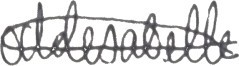
\includegraphics[scale = 15]{my e-sig.jpg}
\end{figure}

DESABELLE, Olyn D.

\noindent\makebox[\linewidth]{\rule{\paperwidth}{0.4pt}}

\section{\textbf{Baa Baa Black Sheep} [50 pts.]}

%Bhabha scattering
%https://www.pas.rochester.edu/assets/pdf/undergraduate/Example_of_Lowest-Order_Processes_in_QED.pdf
%https://www.hep.phy.cam.ac.uk/~thomson/partIIIparticles/handouts/Handout_4_2011.pdf

\begin{figure}[H]
    \centering
    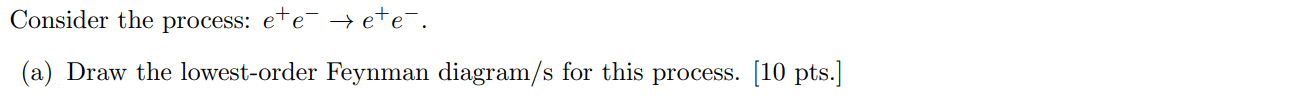
\includegraphics[scale = 0.4]{1a.png}
\end{figure}

There are two lowest-order Feynamn diagrams for this process. One is the pair annihilation $\to$ pair creation represented by an s-channel diagram (left) and the other is the scattering represented by a t-channel diagram (right):

\begin{figure}[H]
    \centering
    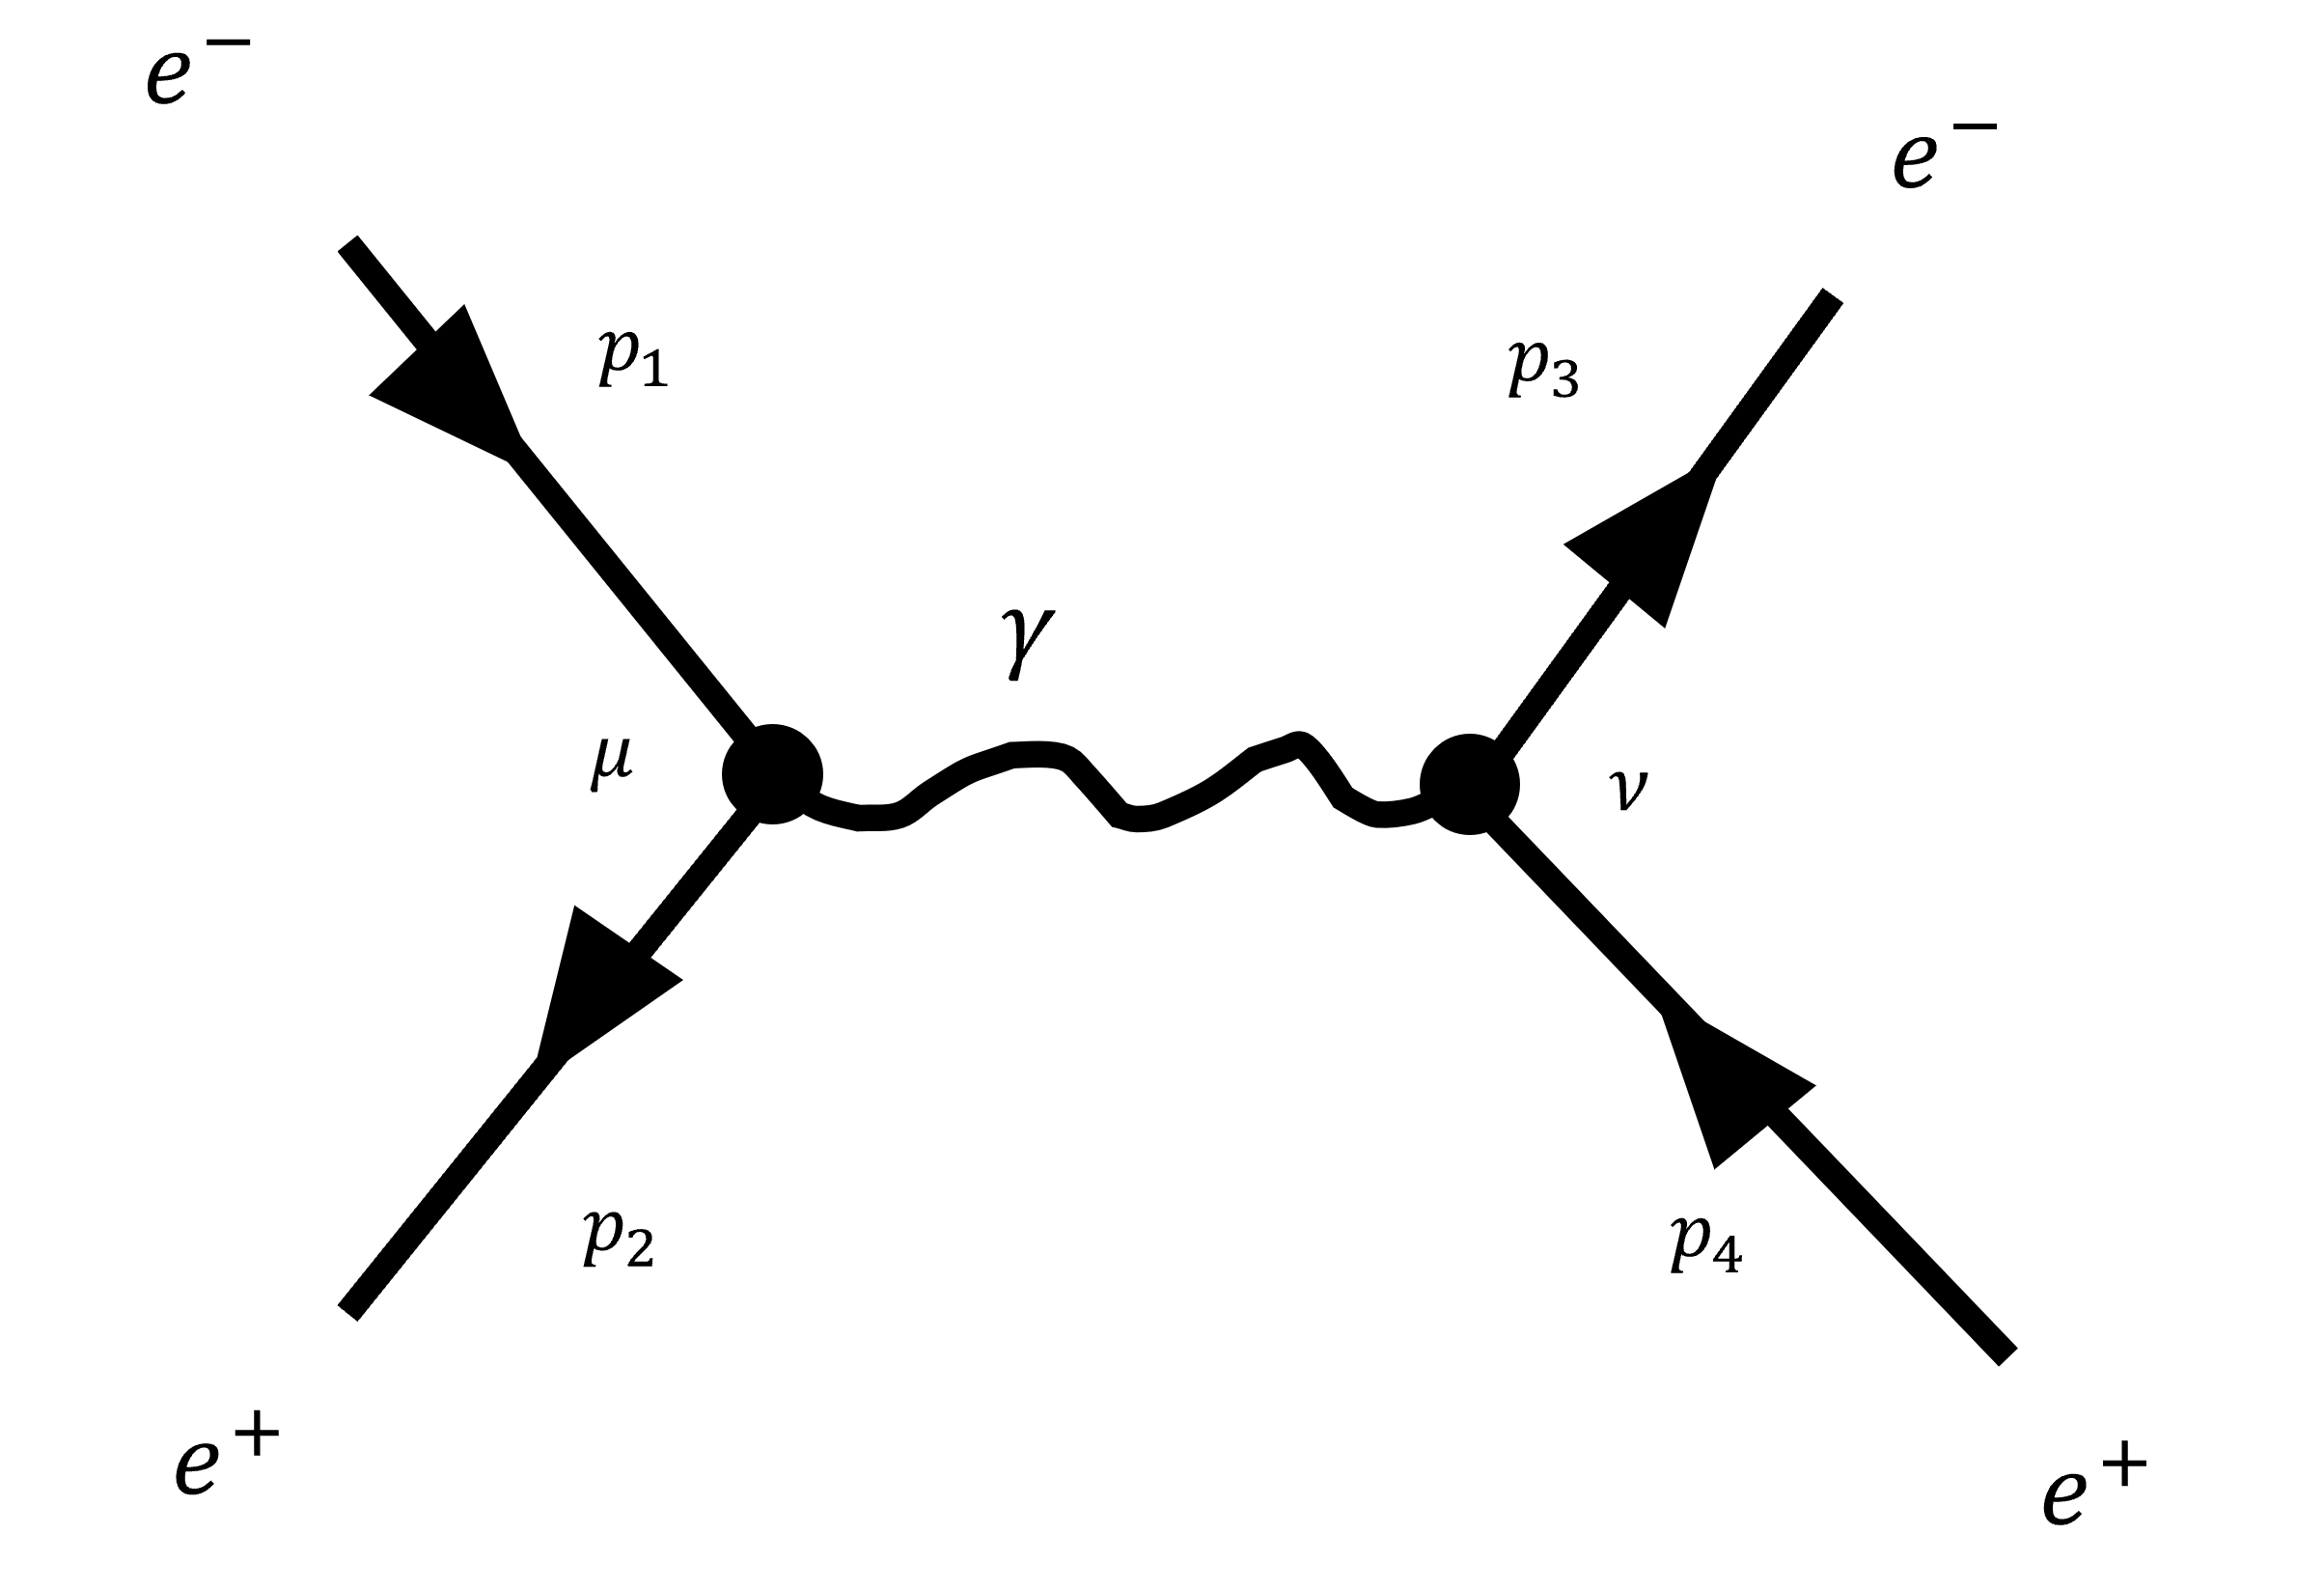
\includegraphics[scale = 0.4]{bhabha s-channel annihilation creation.png}
    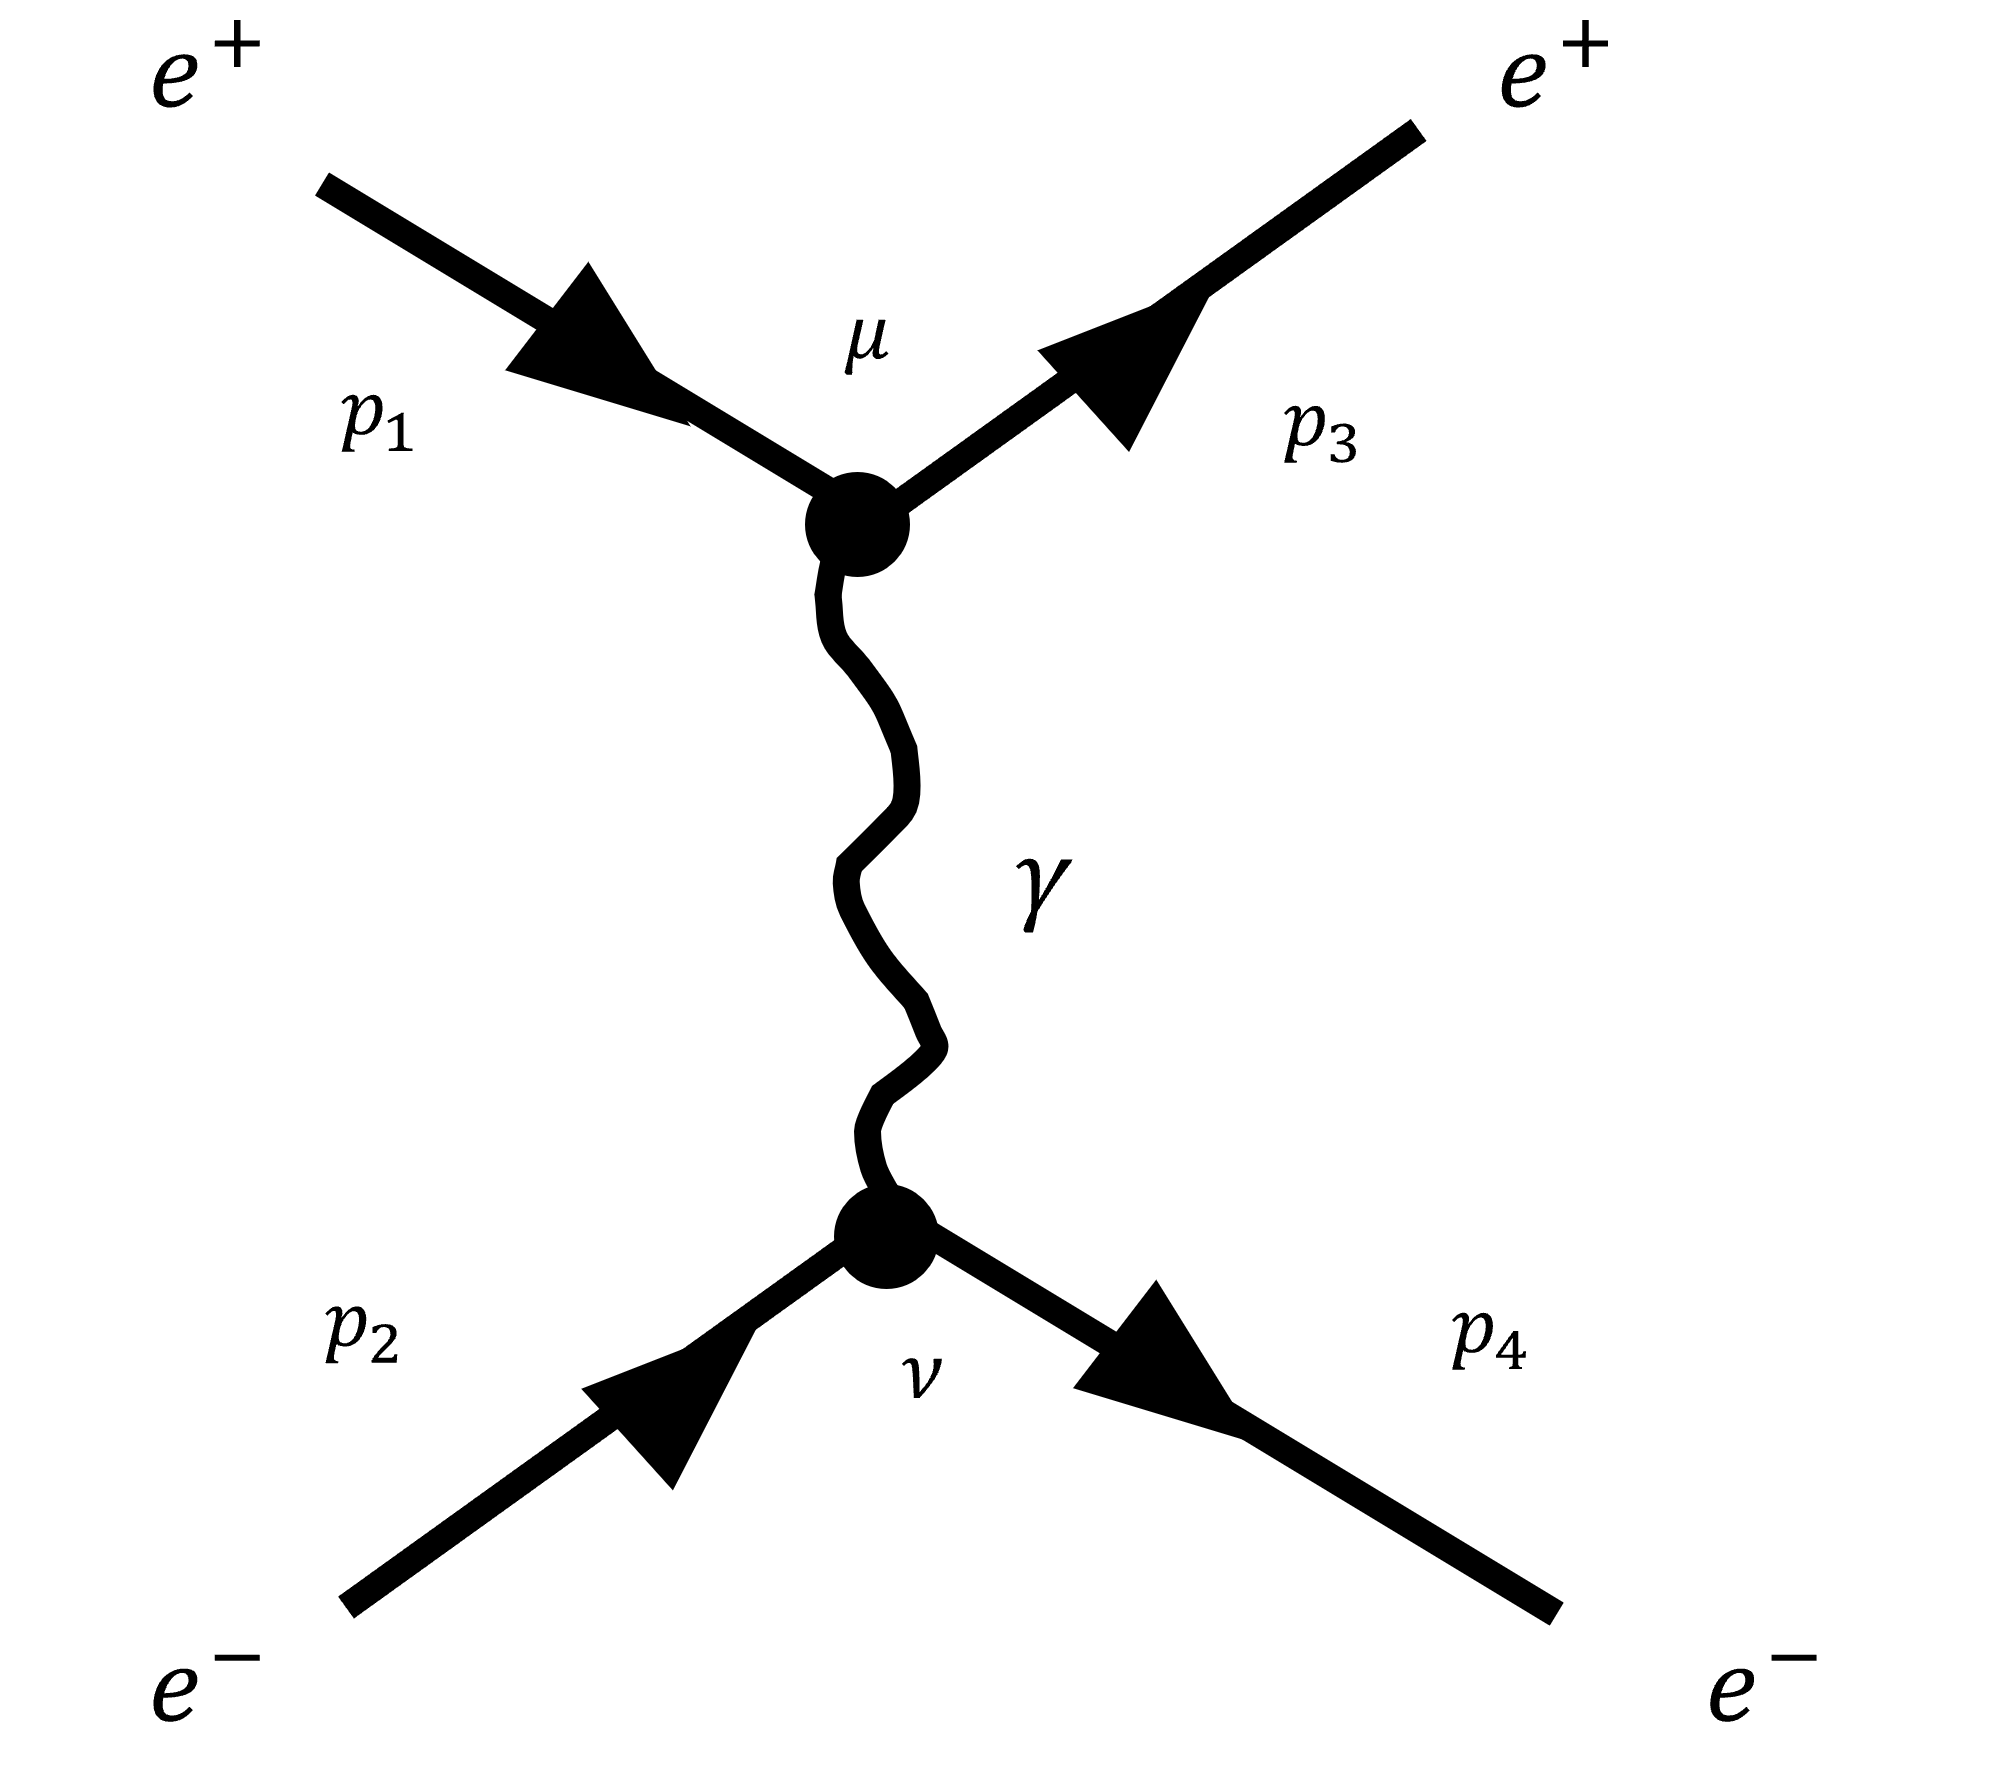
\includegraphics[scale = 0.4]{bhabha t-channel scattering.png}
\end{figure}

%\begin{align} Z =
%\begin{cases}
%    \frac{-a_v  A^2 + a_s A^{5/3} - a_c A^{2/3} -A + a_p A^{1/2}}{-[2 - 2 (a_c A^{2/3})]}& \text{ for even } A,\text{ odd Z}\\
%    \frac{-a_v  A^2 + a_s A^{5/3} - a_c A^{2/3} -A - a_p A^{1/2}}{-[2 - 2 (a_c A^{2/3})]}& \text{ for even } A,\text{ even Z}\\
%    \frac{-a_v  A^2 + a_s A^{5/3} - a_c A^{2/3} -A}{-[2 - 2 (a_c A^{2/3})]}& \text{ for odd } A
%\end{cases}
%\end{align}


%==============================================================
\newpage
%==============================================================



\begin{figure}[H]
    \centering
    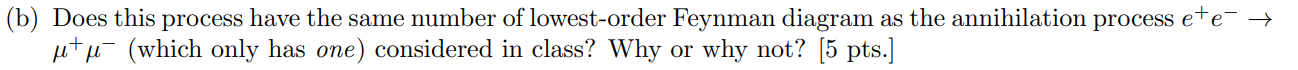
\includegraphics[scale = 0.4]{1b.png}
\end{figure}

The process $e^+e^- \to e^+e^-$ does not have the same number of lowest-order Feynman diagram as the $e^+e^- \to \mu^+\mu^-$ process since the former has 2 while the latter only has 1. This is because in the lowest-order the former can undergo either pair annihilation then pair creation or scattering, while the latter can only undergo pair annihilation.


%==============================================================
\newpage
%==============================================================
\begin{figure}[H]
    \centering
    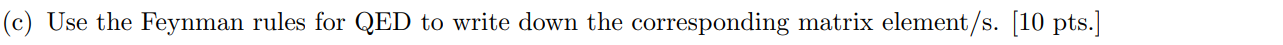
\includegraphics[scale = 0.4]{1c.png}
\end{figure}


We note that the Feynman rules for QED note the following contributions to the matrix element $\mathcal{M}$. We have the following contributions:

\begin{align*}
    \text{initial state particle }(e^{-}) \; &: \; u(p)\\
    \text{initial state antiparticle }(e^{+}) \; &: \; \bar{v}(p)\\
    \text{final state particle }(e^{-}) \; &: \; \bar{u}(p)\\
    \text{final state antiparticle }(e^{+}) \; &: \; v(p)\\
    \text{interaction vertex factor } \; &: \; ie\gamma^{\mu}\\
    \text{photon propagator} \; &: \; -\frac{ig_{\mu\nu}}{q^2}\\
\end{align*}



\underline{s-channel annihilation + creation}

\begin{align}
    -i\mathcal{M}_{s} &= [\bar{v}(p_2)ie\gamma^{\mu}u(p_1)] 
    \left[ \frac{-ig_{\mu\nu}}{q^2} \right]
    [\bar{u}(p_3)ie\gamma^{\nu}v(p_4)]\\
    \mathcal{M}_{s} &= -[\bar{v}(p_2)e\gamma^{\mu}u(p_1)] 
    \left[ \frac{g_{\mu\nu}}{q^2} \right]
    [\bar{u}(p_3)e\gamma^{\nu}v(p_4)]\\
    \mathcal{M}_{s} &= \frac{-e^2}{q^2} [\bar{v}(p_2)\gamma^{\mu}u(p_1)]
    g_{\mu\nu}[\bar{u}(p_3)\gamma^{\nu}v(p_4)]\\
\end{align}

\begin{equation}
\boxed{
    \mathcal{M}_{s} = \frac{-e^2}{q^2} [\bar{v}(p_2)\gamma^{\mu}u(p_1)]
    [\bar{u}(p_3)\gamma_{\nu}v(p_4)]
}
\end{equation}

\underline{t-channel scattering}

\begin{align}
    -i\mathcal{M}_{t} &= [\bar{v}(p_3)ie\gamma^{\mu}v(p_1)] 
    \left[ \frac{-ig_{\mu\nu}}{q^2} \right]
    [\bar{u}(p_4)ie\gamma^{\nu}u(p_2)]\\
    \mathcal{M}_{t} &= -[\bar{v}(p_3)e\gamma^{\mu}v(p_1)] 
    \left[ \frac{g_{\mu\nu}}{q^2} \right]
    [\bar{u}(p_4)e\gamma^{\nu}u(p_2)]\\
    \mathcal{M}_{t} &= \frac{-e^2}{q^2} [\bar{v}(p_3)\gamma^{\mu}v(p_1)]
    g_{\mu\nu}[\bar{u}(p_4)\gamma^{\nu}u(p_2)]\\
\end{align}

\begin{equation}
\boxed{
    \mathcal{M}_{t} = \frac{-e^2}{q^2} [\bar{v}(p_3)\gamma^{\mu}v(p_1)]
    [\bar{u}(p_4)\gamma_{\nu}u(p_2)]
}
\end{equation}
%==============================================================
%\newpage
%==============================================================


%\begin{figure}[H]
%    \centering
%    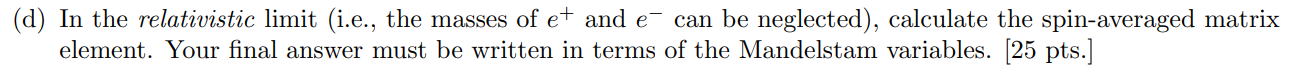
\includegraphics[scale = 0.4]{1d.png}
%\end{figure}

%We may obtain the matrix squared element by combining the two previously obtained matrix elements (written in Mandelstam variables):

%afterwards, we may obtain the spin-averaged matrix element using trace formalism:


%==============================================================
\newpage
%==============================================================

%==============================================================
%we then note that we can switch up the order of differentiation:

\section{\textbf{Look At Me Roll} [50 pts.]}
%============================================================

%Moller scattering

\begin{figure}[H]
    \centering
    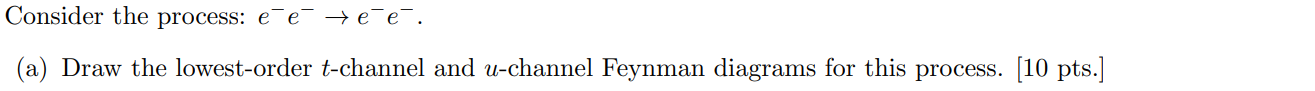
\includegraphics[scale = 0.4]{2a.png}
\end{figure}

The lowest-order t-channel Feynman diagram for the process is given by:

\begin{figure}[H]
    \centering
    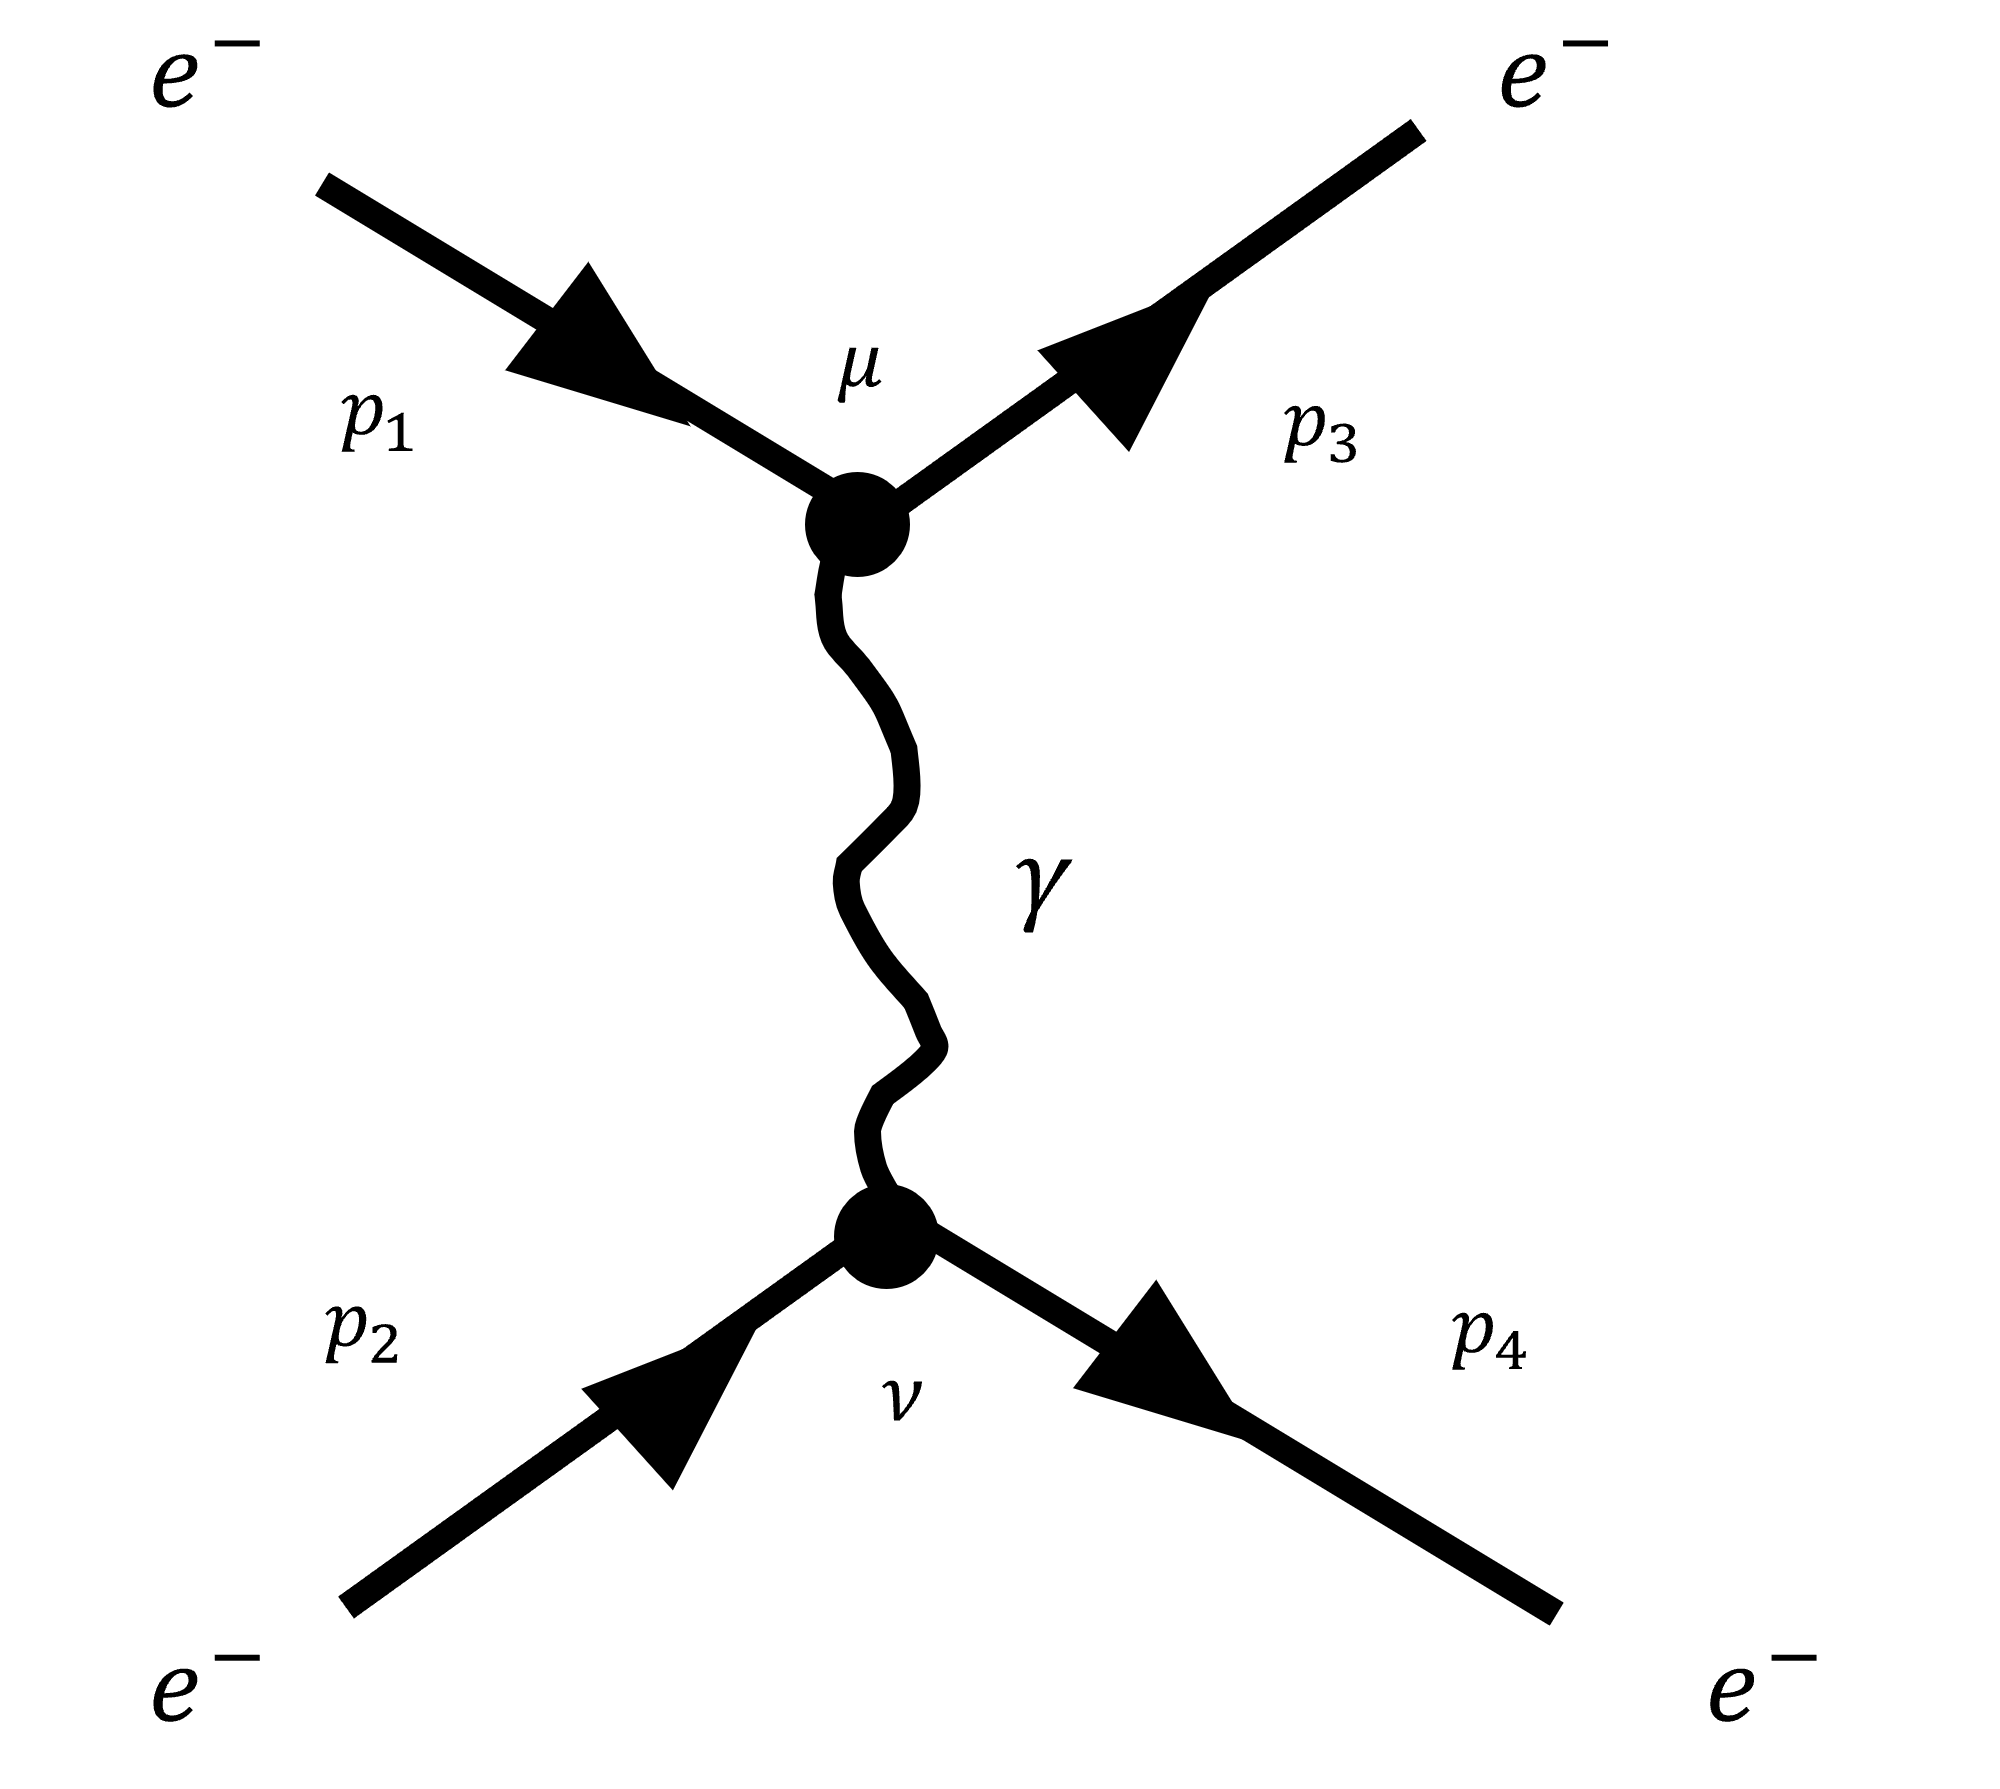
\includegraphics[scale = 0.4]{moller t-channel.png}
\end{figure}


The lowest-order u-channel Feynman diagram for the process is given by:

\begin{figure}[H]
    \centering
    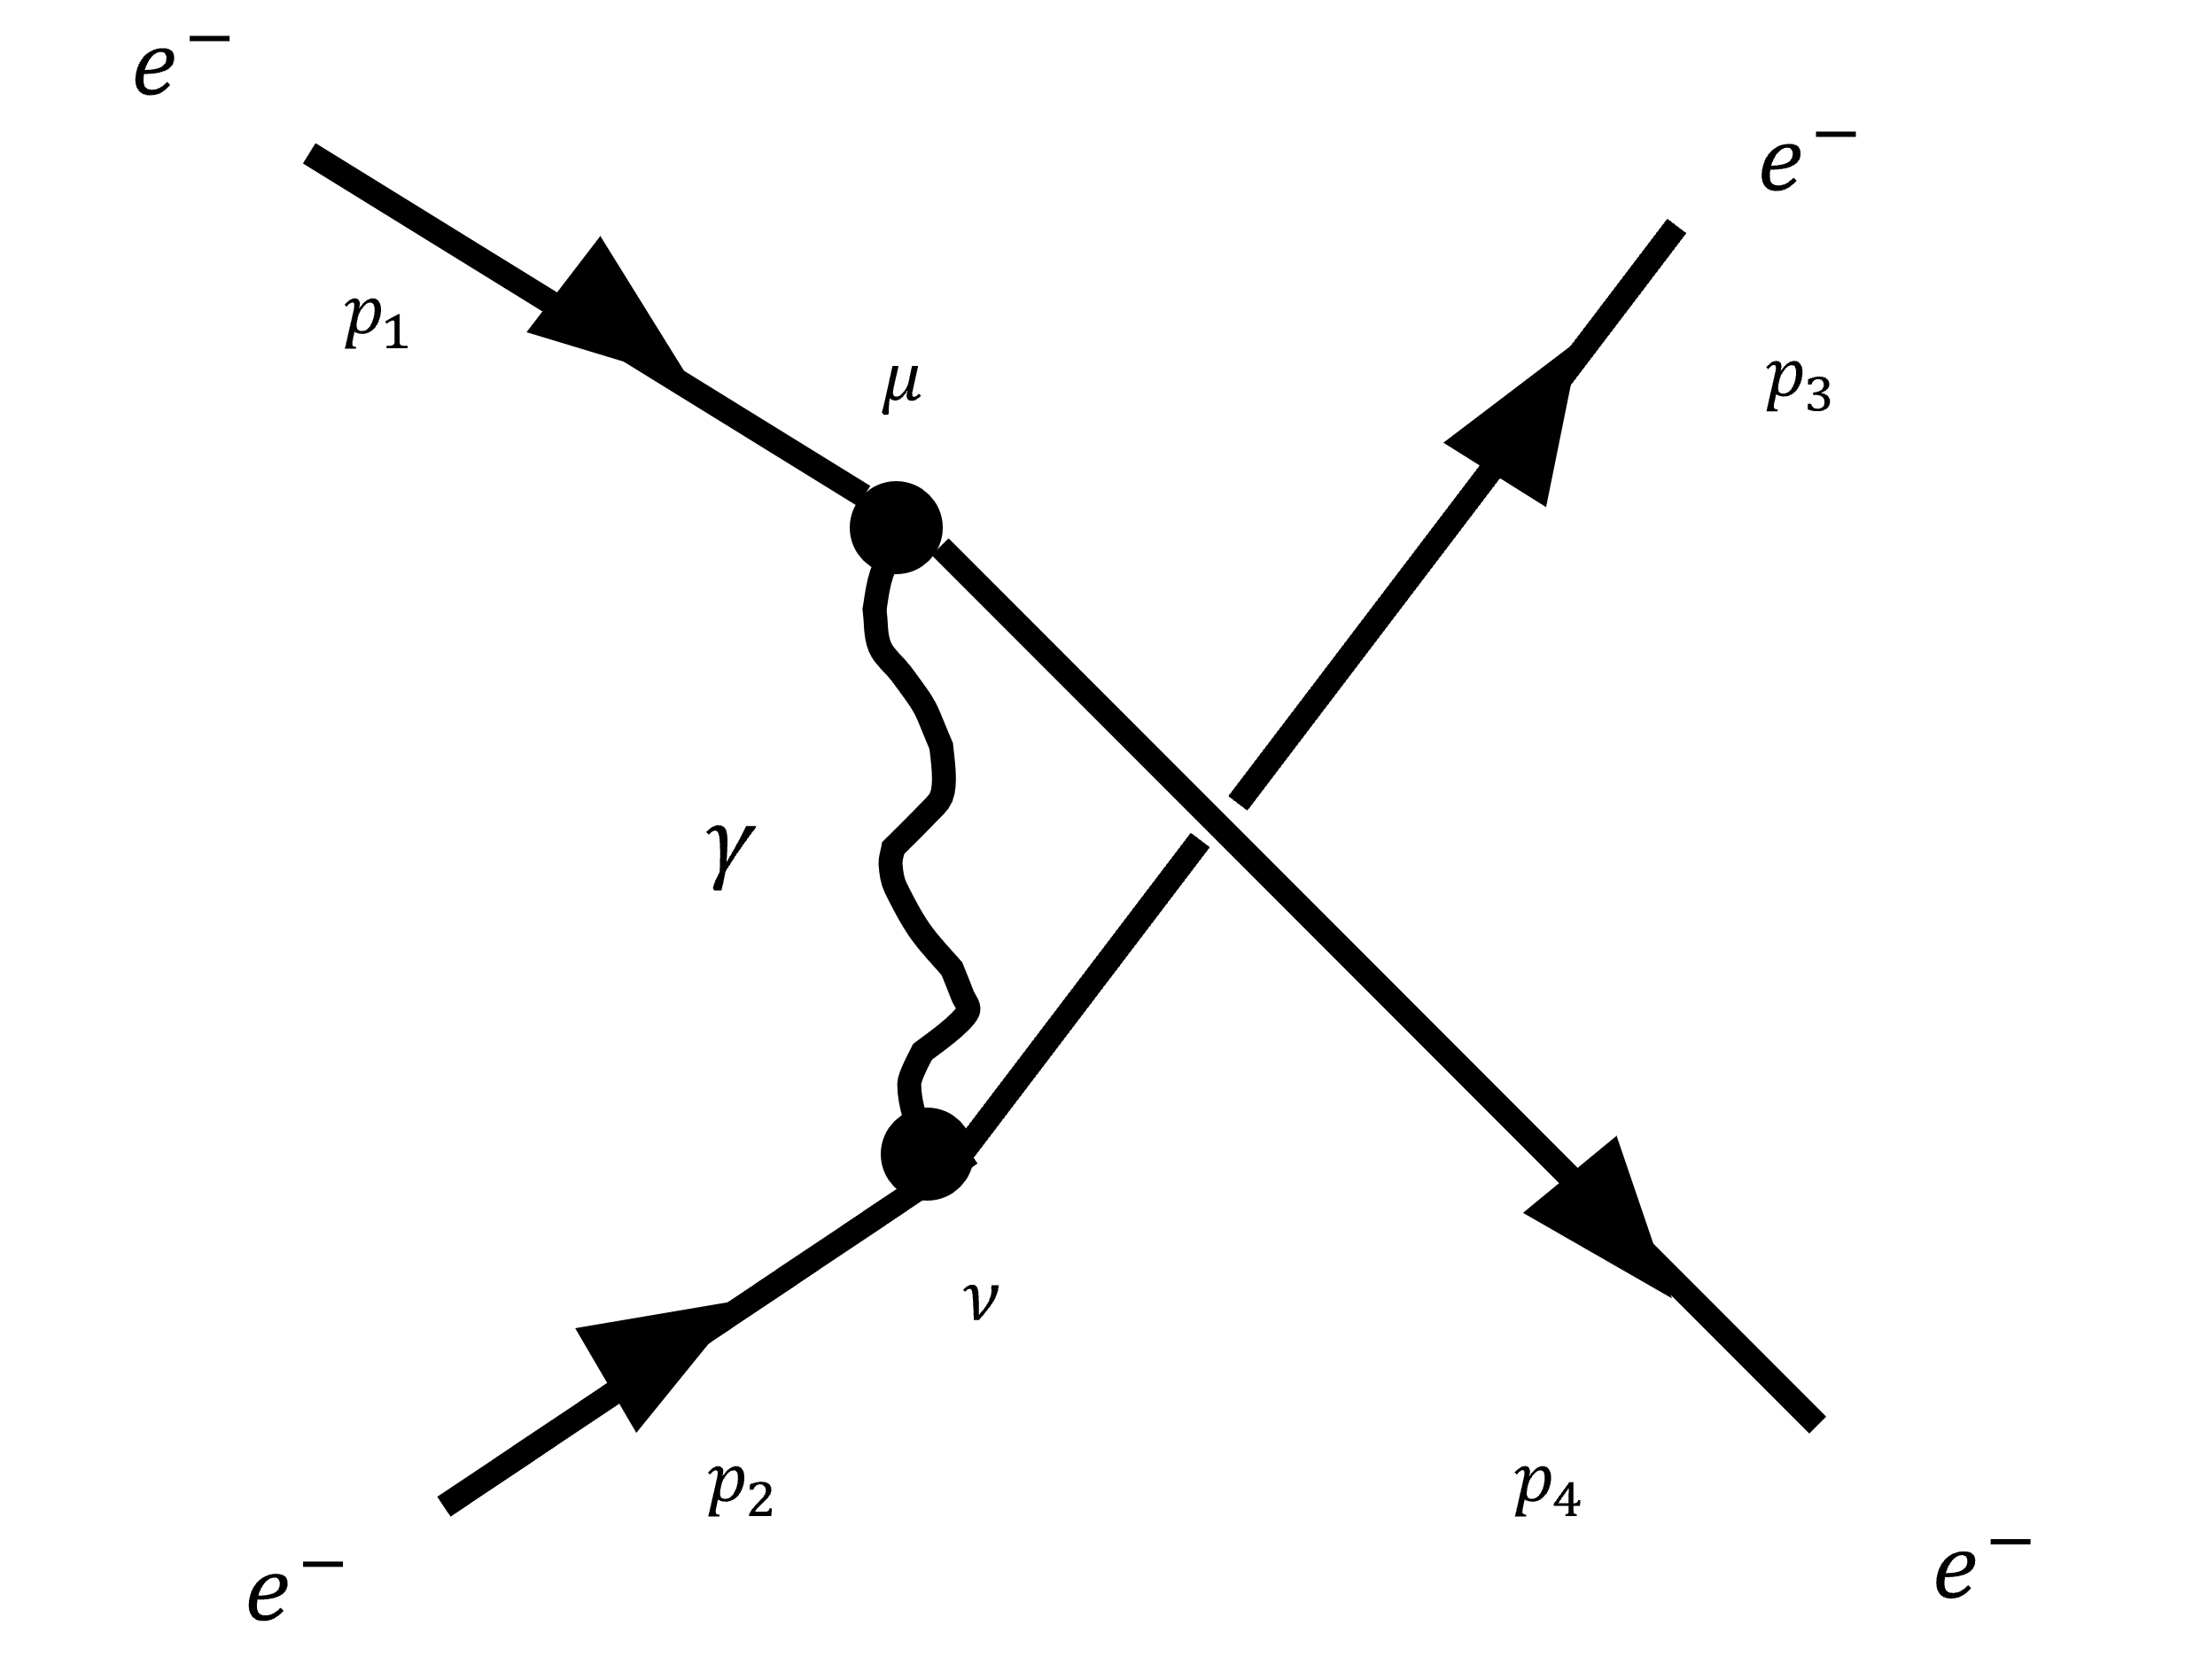
\includegraphics[scale = 0.4]{moller u-channel.png}
\end{figure}

%==============================================================
\newpage
%==============================================================



\begin{figure}[H]
    \centering
    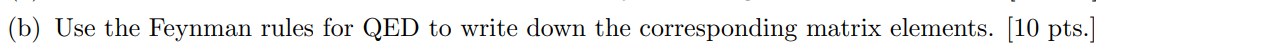
\includegraphics[scale = 0.4]{2b.png}
\end{figure}

\underline{t-channel}

For the t-channel Feynman diagram, the matrix element $\mathcal{M}$ is given by:

\begin{align}
    -i\mathcal{M}_{t} &= [\bar{u}(p_3)ie\gamma^{\mu}u(p_1)] 
    \left[ \frac{-ig_{\mu\nu}}{q^2} \right]
    [\bar{u}(p_4)ie\gamma^{\nu}u(p_2)]\\
    \mathcal{M}_{t} &= -[\bar{u}(p_3)e\gamma^{\mu}u(p_1)] 
    \left[ \frac{g_{\mu\nu}}{q^2} \right]
    [\bar{u}(p_4)e\gamma^{\nu}u(p_2)]\\
    \mathcal{M}_{t} &= \frac{-e^2}{q^2} [\bar{u}(p_3)\gamma^{\mu}u(p_1)]
    g_{\mu\nu}[\bar{u}(p_4)\gamma^{\nu}u(p_2)]\\
\end{align}

\begin{equation}
\boxed{
    \mathcal{M}_{t} = \frac{-e^2}{q^2} [\bar{u}(p_3)\gamma^{\mu}u(p_1)]
    [\bar{u}(p_4)\gamma_{\nu}u(p_2)]
}
\end{equation}

\underline{u-channel}

For the u-channel Feynman diagram, the matrix element $\mathcal{M}$ is given by:

\begin{align}
    -i\mathcal{M}_{u} &= [\bar{u}(p_3)ie\gamma^{\mu}u(p_2)] 
    \left[ \frac{-ig_{\mu\nu}}{q^2} \right]
    [\bar{u}(p_4)ie\gamma^{\nu}u(p_1)]\\
    \mathcal{M}_{u} &= -[\bar{u}(p_3)e\gamma^{\mu}u(p_2)] 
    \left[ \frac{g_{\mu\nu}}{q^2} \right]
    [\bar{u}(p_4)e\gamma^{\nu}u(p_1)]\\
    \mathcal{M}_{u} &= \frac{-e^2}{q^2} [\bar{u}(p_3)\gamma^{\mu}u(p_2)]
    g_{\mu\nu}[\bar{u}(p_4)\gamma^{\nu}u(p_1)]\\
\end{align}

\begin{equation}
\boxed{
    \mathcal{M}_{u} = \frac{-e^2}{q^2} [\bar{u}(p_3)\gamma^{\mu}u(p_2)]
    [\bar{u}(p_4)\gamma_{\nu}u(p_1)]
}
\end{equation}
%==============================================================
%\newpage
%==============================================================


%\begin{figure}[H]
%    \centering
%    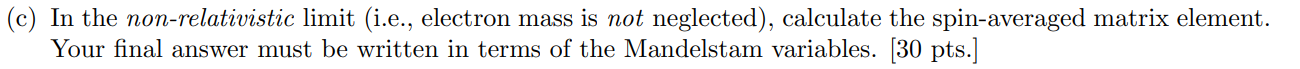
\includegraphics[scale = 0.4]{2c.png}
%\end{figure}


%==================================
%helpful ps8 and ps9
\end{document}